\documentclass[twoside,10pt]{article}
\usepackage{/Users/bradenhoagland/latex/styles/toggles}
%\toggletrue{sectionbreaks}
%\toggletrue{sectionheaders}
\newcommand{\docTitle}{Math 611 - HW 4}
\usepackage{/Users/bradenhoagland/latex/styles/common}
\importStyles{modern}{rainbow}{boxy}

%\renewcommand{\theenumi}{\alph{enumi}}

\begin{document}
%\tableofcontents

% ------------------------------
% 1.2: 12
% ------------------------------
\begin{exer}[1.2: 12]
Klein bottle in $\mathbb{R}^{3}$.
\end{exer}

\begin{enumerate}
	\item To represent the Klein bottle in $\mathbb{R}^{3}$, we can take the cylinder pictured below and attach the two boundary circles together with opposite orientations, as normal; however, we must also identity the two dashed circles, as they intersect.

		\begin{figure}[H]
			\centering
			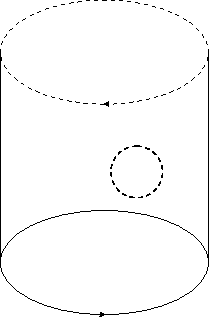
\includegraphics[scale=0.8]{fig/12a.pdf}
			%\caption{}
		\end{figure}

		We can draw this as the square below, where the edge $c$ is necessary only because without it, the light gray area outside the dark gray central 2-cell is not actually a 2-cell (it's not a disk).

		\begin{figure}[H]
			\centering
			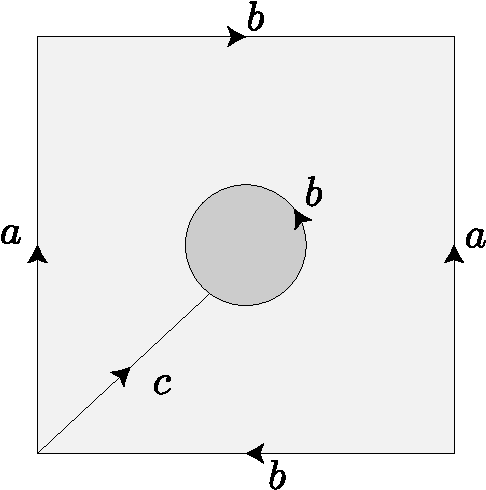
\includegraphics[scale=0.6]{fig/12b.pdf}
			%\caption{}
		\end{figure}

		Note that all 5 vertices in the above figure are actually the same point, so there are 3 unique loops centered at it ($a, b,$ and $c$). Thus the 1-skeleton has fundamental group $\pi_1(S^{1}\vee S^{1}\vee S^{1}) \cong \ang{a,b,c}$. Adding in both 2-cells gives us the fundamental group of the whole space:
		\[
			\pi_1(X) = \ang{a,b,c \;|\; aba^{-1}bcbc^{-1}, b} = \ang{a,b,c}.
		\] 

	\item To find the fundamental group of $Y$ instead, we just need to delete the dark gray inner 2-cell from the above square diagram. This amounts to removing the relation $b=1$ from the fundamental group, so
		\[
			\pi_1(Y) = \ang{a,b,c \;|\; aba^{-1}bcbc^{-1}}.
		\] Note that visually, the book's comment about $\varepsilon=\pm 1$ makes sense, as the orientation of the inner $b$ in the square diagram is arbitrary.

	\item We will first show this result for $S^{3}-Z$ instead. We can cut the Klein bottle with a disk (see the blue portion of attached figure 1), naturally dividing $S^{3}-Z$ into a part inside the Klein bottle and a part outside.

		The inside is a just a solid torus, and there is a clear deformation retract from it onto $Y$ (see attached figure 2).

		Since the compliment in $S^{3}$ of a solid torus is just another solid torus, the outside portion of $S^{3}-Z$ has the same deformation retract onto $Y$. Thus all of $S^{3}-Z$ deformation retracts onto $Y$, so $\pi_1(S^{3}-Z) \cong \pi_1(Y)$.

		Now we show that $S^{3}-Y$ and $\mathbb{R}^{3}-Y$ have the same fundamental groups. Since $S^{3}-Z = (\mathbb{R}^{3}-Z) \uni D^{3}$ and since these two sets have intersection $D^{3}- \left\{ \text{the point at infinity} \right\} \simeq S^{2}$ (which is simply connected), we can apply Van Kampen's Theorem to get $\pi_1(S^{3}-Z) \cong \pi_1(\mathbb{R}^{3}-Z) * \pi_1(D^{3}) \cong  \pi_1(\mathbb{R}^{3}-Z)$. Our earlier results then show $\pi_1(\mathbb{R}^{3}-Z) \cong \pi_1(Y)$.
\end{enumerate}

\newpage

% ------------------------------
% 1.2: 22
% ------------------------------
\begin{exer}[1.2: 22]
Wirtinger presentation.
\end{exer}

\begin{enumerate}
	\item Suppose we have not yet added all the extra squares $S_{\ell}$. We can fix a point in the plane and form loops around each of the reactangular strips $R_{i}$ (see attached figure 3). This means the fundamental group of the space $X - \left\{ S \right\}_{\ell}$ is $*_{i=1}^{n}\mathbb{Z}$, where $n$ is the total number of strips.

		Now choose the orientation as on the knot as pictured, then use the right hand rule to orient each loop. Then when we add in each square, we get the situation pictured below, giving us relations of the form $x_i x_j^{-1} x_i^{-1} x_k=1$.

		\begin{figure}[H]
			\centering
			\includegraphics[scale=1]{fig/22b.pdf}
			%\caption{}
		\end{figure}

		Thus the fundamental group of $X$ is
		\[
			\ang{ \left\{ x_i \right\} \;|\; \{x_i x_j^{-1} x_i^{-1} x_k\} } = \ang{ \left\{ x_i \right\} \;|\; \left\{ x_i x_j x_i^{-1} = x_k \right\}},
		\] 
		as desired. Since $X$ is a deformation retract of $\mathbb{R}^{3}-K$, this is also the fundamental group of $\mathbb{R}^{3}-K$, as desired.

	\item When we abelianize this group, all the relations simplify to $x_{j}=x_{k}$. This makes all the generators become the same, i.e.
		\[
			\text{ab}(\pi_1(\mathbb{R}^{3}-K)) \cong \ang{x_1}\cong \mathbb{Z}.
		\] 
\end{enumerate}

\newpage

% ------------------------------
% 3
% ------------------------------
\begin{exer}
	Wirtinger Presentation of $(2,n)$ torus knot.
\end{exer}

Suppose we have a $(2,n)$ torus knot $K$. Label the knots as follows.

\begin{figure}[H]
	\centering
	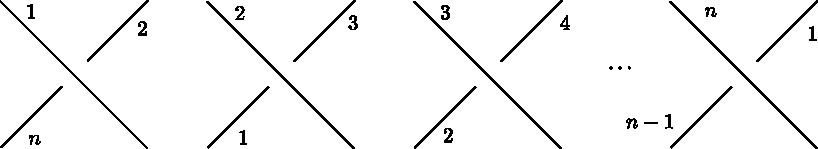
\includegraphics[scale=1]{fig/3a.pdf}
	%\caption{}
\end{figure}

The Wirtinger presentation for $K$ then has the following generators and relations.
\begin{center}
\begin{tabular}{c | c}
	Generators & Relations \\
	\hline
	$x_1$ & $x_1 x_n x_1^{-1} = x_2$ \\
	$x_2$ & $x_2 x_1 x_2^{-1} = x_3$ \\
	$\vdots$ & $\vdots$ \\
	$x_i$ & $x_1 x_{i-1} x_{i}^{-1} = x_{i+1}$ \\
	$\vdots$ & $\vdots$ \\
	$x_{n-1}$ & $x_{n-1}x_{n-2}x_{n-1}^{-1}=x_{n}$ \\
	$x_n$ & $x_{n}x_{n-1}x_{n}^{-1}= x_1$
\end{tabular}
\end{center}
We can now reduce this system to one involving only $x_1$ and $x_2$. Begin by subsituting into all other relations $x_{n}= x_{n-1}x_{n-2}x_{n-1}$, then repeat for the $x_{n-1}, x_{n-2}, \dots, x_{3}$ relations. We have
\begin{align*}
	x_{2} &= x_1 (x_{n-1}x_{n-2}x_{n-1}^{-1}) x_1^{-1} \\
	      &= x_1 (x_{n-2}x_{n-3}) (x_{n-2}x_{n-3}^{-1}x_{n-2}^{-1}) x_{1}^{-1} \\
	      &= \quad\vdots \\
	      &= (x_1x_2)^{(n-1)/2} x_1 (x_2^{-1}x_1^{-1})^{(n-1)/2} \\
	(x_2x_1)^{(n-1)/2} x_2 &= (x_1x_2)^{(n-1)/2} x_1.
\end{align*}

The relation $x_{n}x_{n-1}x_{n}=x_1$ reduces to the same equation, so we only need this one relation. Thus the Wirtinger presentation becomes
\[
	\pi_1(\mathbb{R}^{3}-K)	\cong \ang{x_1, x_2 \;|\; (x_1x_2)^{(n-1)/2}x_1 = (x_2x_1)^{(n-1)/2}x_2}.
\] Note that this formula only works when $n$ is odd, since otherwise $(n-1)/2$ is not an integer. Let $x=(x_1x_2)^{(n-1)/2}x_1$ and $y = x_2x_1$, then this relation gives
\begin{align*}
	x^2 &= (x_1x_2)^{(n-1)/2}x_1 \cdot (x_1x_2)^{(n-1)/2}x_1 \\
	    &= (x_2x_1)^{(n-1)/2}x_2 \cdot (x_1x_2)^{(n-1)/2}x_1 \\
	    &= (x_2x_1)^{n} \\
	    &= y^{n}.
\end{align*}
Thus $\pi_1(\mathbb{R}^{3}-K) \cong \ang{x,y \;|\; x^{2}=y^{n}}$, as desired.

\newpage

% ------------------------------
% 1.3: 4
% ------------------------------
\begin{exer}[1.3: 4]
Simply connected covering spaces.
\end{exer}

\begin{enumerate}
	\item \textbf{Union of sphere and diameter:} A covering space of this is an infinite line of spheres joined by line segments, with covering map shown in attached figure 4.

	\item \textbf{Union of sphere and circle intersecting at 2 points:} Now we need every sphere to be attached to four other spheres instead of two. The general idea is the same, with many infinitely branching chains of spheres (no branches every join up in order to keep the space simply connected). See attached figure 5.
\end{enumerate}

\newpage

% ------------------------------
% 1.3: 7
% ------------------------------
\begin{exer}[1.3: 7]
	Show that $\pi_1(Y)$ is trivial and that $f$ doesn't have a lift.
\end{exer}

Let $A$ be the $y$-axis component, $B$ the sine curve graph, and $C$ the connecting arc of $Y$ (see attached figure 6).

\begin{enumerate}
	\item \textbf{Trivial fundamental group:} Since $Y$ is path connected, we can choose any point to be the basepoint. Let $a \in A$. The topologist's since curve is known to not be path connected, so any loop based at $a$ cannot pass from $A$ to $B$ (and vice versa) unless it travels through $C$. But this means that no loop at $a$ can wind fully around $Y$, so all loops at $a$ are nullhomotopic. Thus $\pi_1(Y) = 1$.

	\item \textbf{$f$ doesn't have a lift:} Suppose a lift $\tilde{f}$ of $f$ exists such that the following diagram commutes.
		\[
			\begin{tikzcd}
			& \mathbb{R} \dar{p = e^{2\pi it}} \\
			Y \arrow[ur, "\tilde{f}"] \rar["f"'] & S^{1}
			\end{tikzcd}
		\] 

		Model $S^{1}$ by the set $\left\{ z \in \mathbb{C} \;|\; |z|=1 \right\}$, then without loss of generality, suppose $f(A) = 1 \in S^{1}$. We then know $p^{-1}(f(A)) = \mathbb{Z}$, so we can suppose (again without loss of generality) that $\tilde{f}(A) = 0$. This forces $\tilde{f}(Y-A) = (0,1)$.

		Now consider the open set $U = (-\varepsilon,\varepsilon) \subset \mathbb{R}$, where $\varepsilon$ is small (say $< 1/2$). Then $\tilde{f}^{-1}(U)$ is composed of $A$ plus a small region $C$ to the left of $A$ (see attached figure 7); however, since $Y$ has the subspace topology with respect to $\mathbb{R}^{2}$ and any open ball in $\mathbb{R}^{2}$ containing $A$ must also intersect some of $B$, we know $U$ cannot be open in $Y$. Thus $\tilde{f}$ is not continuous, a contradiction. This means $\tilde{f}$ could not have existed in the first place.
\end{enumerate}

\newpage

\end{document}
